\chapter{Related Literature}
\begin{quote} 
\textit{This section explores contemporary academic/scientific papers and articles that establish the research context necessary for the thesis.} 
\end{quote}


  
\section{Dye-Sensitized Solar Cells(DSCs)}

The basic structure of \ac{DSCs} is represented in the Figure ~\ref{fig:DSC_struc}. 

\begin{figure}[H]
\begin{center}
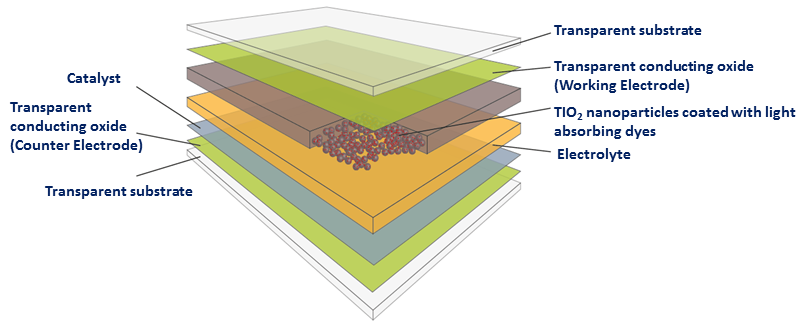
\includegraphics[width=\textwidth]{images/DSCs_struc}
\caption{Structure of a DSC (adapted from \cite{exeger_cell_sand}) }
\label{fig:DSC_struc}
\end{center}
\end{figure}

The most commonly used substrate is glass coated with \ac{FTO}. Attached to the surface of the nano-crystalline particles of Titanium dioxide(\ce{TiO2}) is a mono-layer of the light-sensitive-charge-transfer dye. The dye absorbs photons of incoming light and uses this energy to release free electrons to the \ce{TiO2} layer acting as the \ac{WE} and then onto metal contacts. An electrolyte is filled between the electrodes and helps transfer electrons from the \ac{CE} to the dye particle (which is in an oxidised state due to a loss of electron) to reduce it back to its ground state. The most commonly used redox couple and the one that gives the best cell efficiencies when combined with \ce{TiO2}, is iodide/triiodide (\ce{I-}/\ce{I3-}). The oxidised dye gets electrons from the iodide ions which, in turn, get oxidised to triiodide in the process. The triiodide ions then diffuse to the counter electrode, where they get reduced back to iodide by the electrons returning from the external load. Thus, the cell operation is based on consecutive reduction/oxidation cycles and, in an ideal cell, no chemical substances are permanently transmuted. The most often used counter electrode catalyst for the triiodide/iodide reduction reaction is platinum, though also carbon materials and certain conductive polymers have been successfully employed in this function.\\
\begin{figure}[H]
\begin{center}
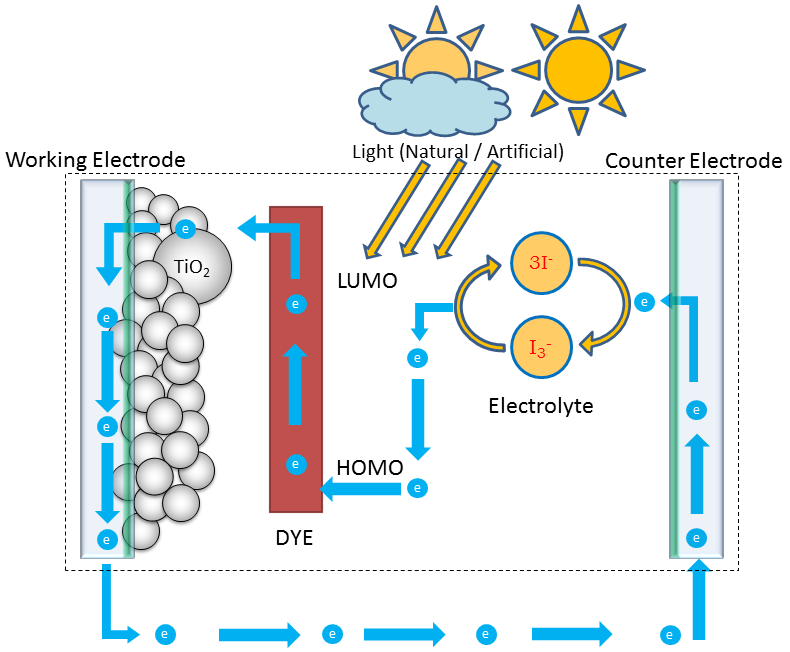
\includegraphics[width=\textwidth]{images/Cell_Cycle}
\caption{ The structure and operating principle of a DSC (adapted from \cite{toivola2010dye,}\cite{gcell_DSSC_cycle})}
\label{fig:Cell_Cycle}
\end{center}
\end{figure}

The amount of current that the cell is able to generate is determined by the energetic distance of the \ac{HOMO} and \ac{LUMO} of the dye, which equals the band gap in inorganic semiconductors. The maximum voltage, on the other hand, is defined as the difference between the redox level of the electrolyte and the Fermi level of the \ce{TiO2}.With iodide/triiodide redox couple, this difference is 0.9 V, though slight variation is caused by the electrolyte composition due to species adsorbed on the \ce{TiO2} surface, which may somewhat alter the Fermi level position. Also, there is always some recombination in the cell which lessens the amount of electrons in the TiO2 film, thus lowering the Fermi level and decreasing the cell voltage. \cite{toivola2010dye}.  This operating principle of \ac{DSCs} is depicted in the Figure ~\ref{fig:Cell_Cycle} on page ~\pageref{fig:Cell_Cycle}. \\


  
  
\subsection{Single diode model}\label{sec:SDM}
The simplest equivalent circuit of a generic solar cell is a Single diode model comprising of a current source in parallel with a diode.A slightly more detailed model includes a shunt resistance of the cell which takes into account the parallel resistive losses representing leakage current across the junction in the cell. This model is sometimes referred to as a single exponential five-parameter model\cite{vignati2012solutions}. The incident photons induces a current in the active area that is proportional to the intensity of the light falling on the cell.

 \begin{figure}[H]
  \begin{center}
  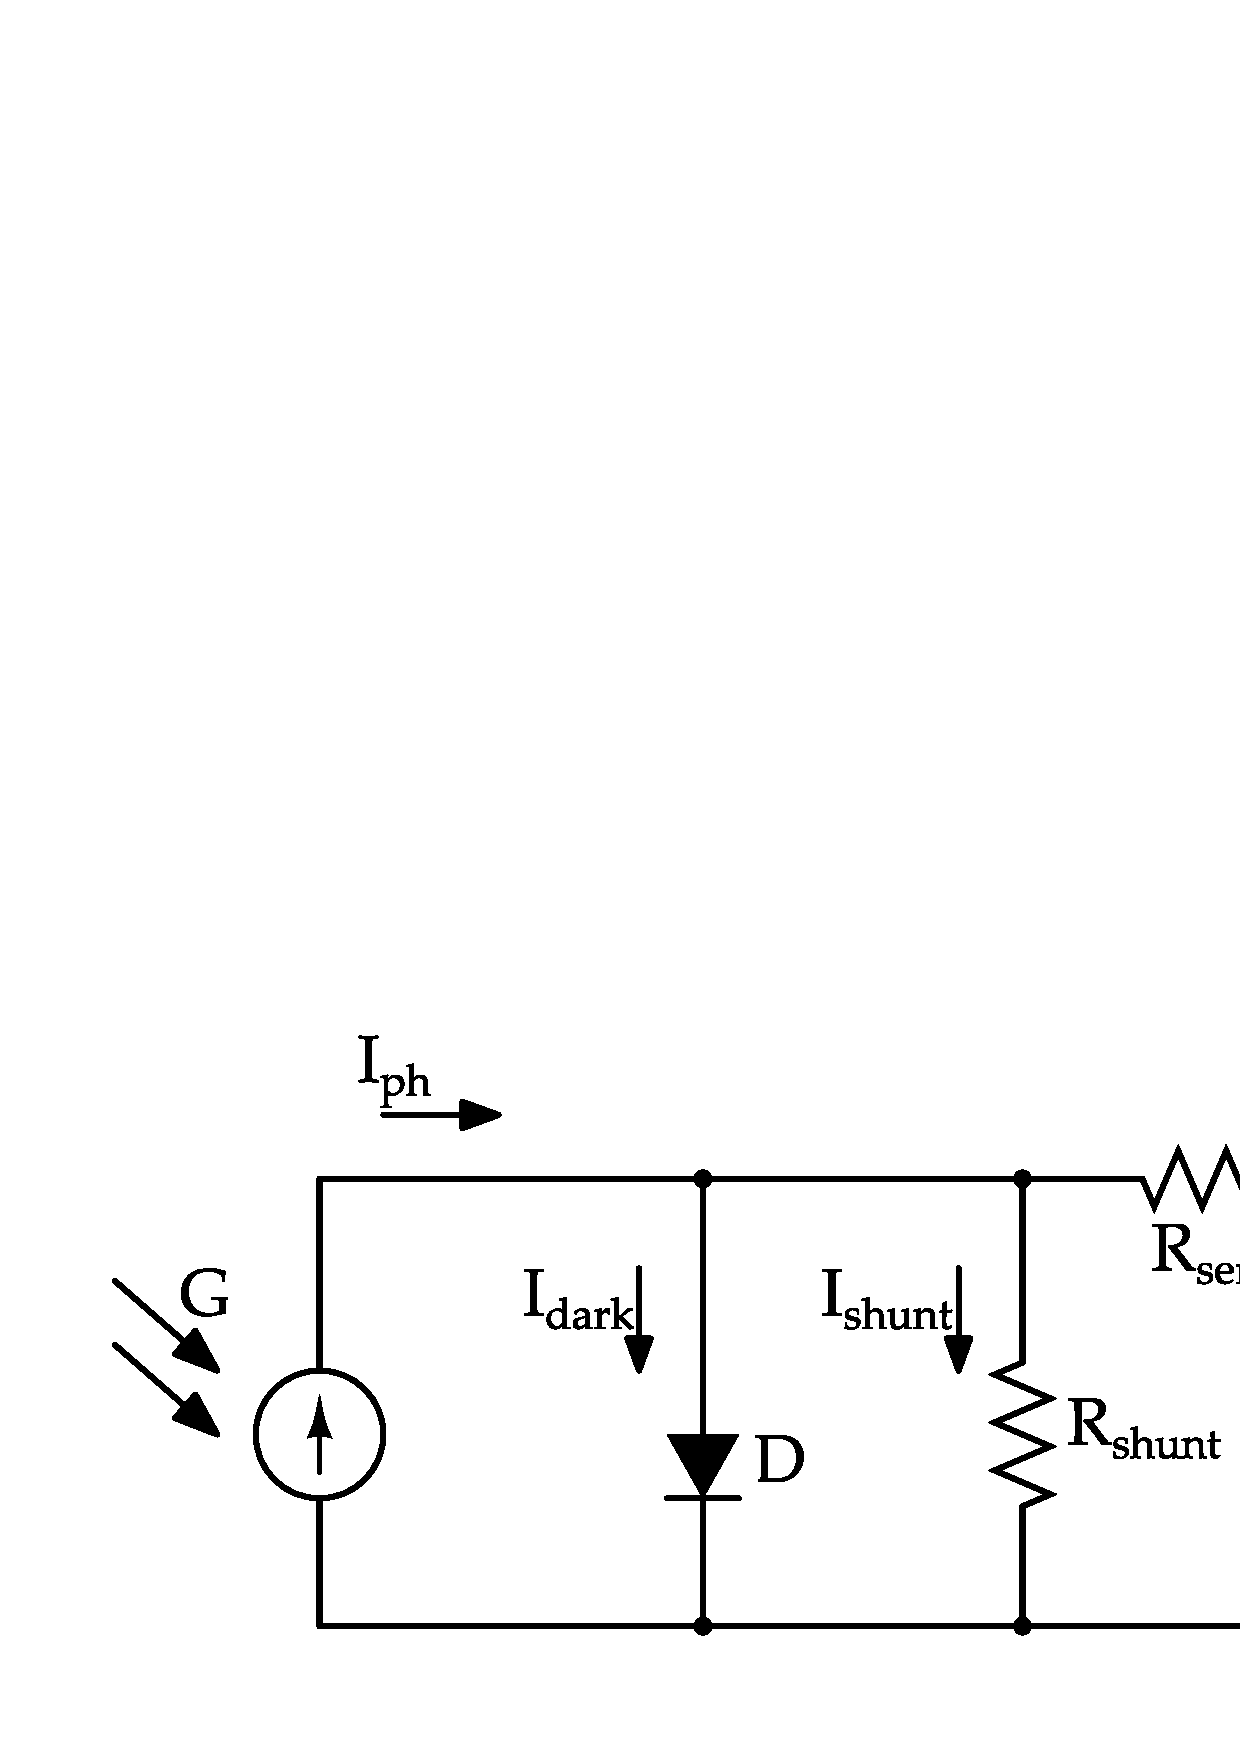
\includegraphics[width=\textwidth]{images/simplified_single_diode_model}
  \caption{ Single diode model for a solar cell }
  \label{fig:EQu_cell}
  \end{center}
  \end{figure}
  
% % % %**Change text**  
The power conversion efficiency of a solar cell is determined from the current versus applied voltage (I-V ) characteristics under illumination. The I-V curve and device efficiency are reported with respect to a standard reference spectral irradiance distribution, the air mass 1.5 global (AM 1.5G) spectrum\cite{wenger2010strategies}. The I-V characteristics of a solar cell are well described by an equivalent electric circuit in Figure ~\ref{fig:EQu_cell} on page ~\pageref{fig:EQu_cell} . Under illumination, a constant photo current (I\textsubscript{ph}) is generated. If a forward voltage bias is applied, a dark diode current (I\textsubscript{dark}) flows in the opposite direction. A shunt resistance (R\textsubscript{shunt}) may arise from charge recombination in the photo-active layer and induce a shunting current(I\textsubscript{shunt}).The series resistance (R\textsubscript{series}) includes the contact resistance at interfaces, the bulk resistance and the sheet resistance of the transparent electrodes. The total measured current then is:
 
 \begin{equation}
 \begin{aligned}
  I = I\textsubscript{ph} - I\textsubscript{dark} - I\textsubscript{shunt} = I\textsubscript{ph} -  I\textsubscript{s} (e^{\frac{eV}{\textit{mk}T}}-1) - \dfrac{V+IR\textsubscript{series}}{R\textsubscript{shunt}}
   \label{eq:equ_current}
   \end{aligned}
   \end{equation}

 where \textbf{I\textsubscript{s}} is the diode saturation current, \textbf{V} is the applied bias voltage, \textbf{\textit{m}} is an ideality factor ( \textit{m} = 1 for an ideal cell), \textbf{\textit{k}} is the Boltzmann constant, and \textbf{T} is the device temperature\cite{wenger2010strategies}. For small forward bias voltages the numerical value of the exponential is very large and 
  the thermal voltage very small, therefore the '-1' in the diode equation can be safely neglected and the forward diode current can be written as\cite{pv_education_org}:
  \begin{equation}
   \begin{aligned}
    I\textsubscript{dark}= I\textsubscript{s} (e^{\frac{eV}{\textit{mk}T}}) 
    \label{eq:equ_current_dark}
    \end{aligned}
   \end{equation}
   
   Substituting the value of I\textsubscript{dark} back in equation ~\ref{eq:equ_current} and neglecting the shunt resistance we can simplify the equation to as below (equation ~\ref{eq:equ_new_cell_current}). This can be schematically depicted as Figure ~\ref{fig:simple_EQu_cell} on page ~\pageref{fig:simple_EQu_cell}. The simplified equation suffices for most modelling applications.
   
    \begin{equation}
    \begin{aligned}
     I = I\textsubscript{ph} - I\textsubscript{dark} - I\textsubscript{shunt} = I\textsubscript{ph} -  I\textsubscript{s} (e^{\frac{eV}{\textit{mk}T}})
      \label{eq:equ_new_cell_current}
      \end{aligned}
      \end{equation}
  
     
 \begin{figure}[H]
   \begin{center}
   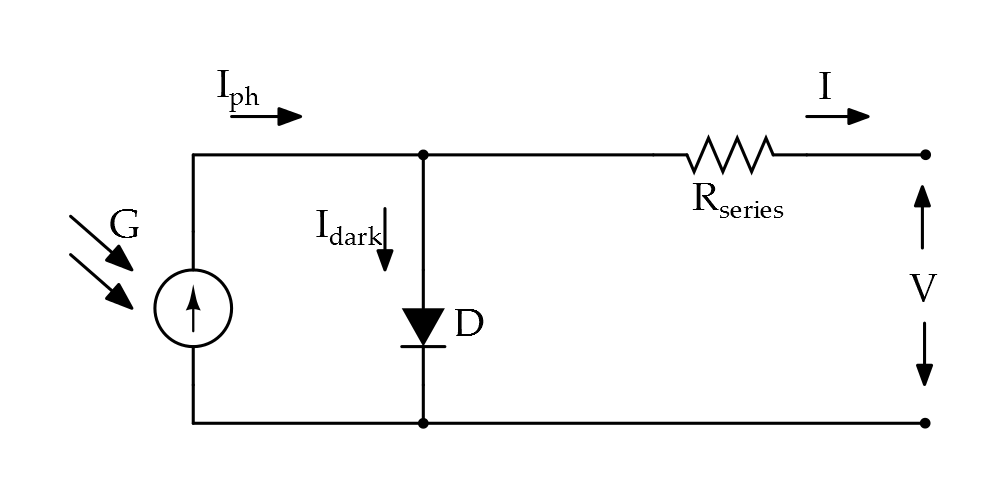
\includegraphics[width=\textwidth]{images/simplified_single_diode_model_simple}
   \caption{ Simplified single diode model for a solar cell }
   \label{fig:simple_EQu_cell}
   \end{center}
   \end{figure}

The maximum-power operating point defines the condition at which the power output (P\textsubscript{\textit{max}} = I\textsubscript{\textit{max}}V\textsubscript{\textit{max}}) of the device is maximal.
The so-called \ac{F.F} is often used to characterise the maximum power ,

\begin{equation}
 \begin{aligned}
  \ac{F.F} = \dfrac{I\textsubscript{\textit{max}}V\textsubscript{\textit{max}}}{I\textsubscript{\textit{sc}}V\textsubscript{\textit{oc}}}
   \label{eq:equ_current_new}
   \end{aligned}
   \end{equation}
   
The accuracy and complexity of the model can be increased by including Temperature dependence of the photo current and diode saturation current; shunt resistance in parallel with the diode and accommodating for variance in the quality factor of the diode either by having a variable parameter or introduction of an additional diode into the circuit as done in the Double Diode Model.


\subsection{Double diode model}\label{sec:DDM}

The single diode equation assumes a constant value for the ideality factor \textit{n}. In reality, the ideality factor is a function of voltage across the device. At high voltages, when the recombination in the device is dominated by the surfaces and the bulk regions, the ideality factor is close to one. However at lower voltages, recombination in the junction dominates and the ideality factor approaches two. The junction recombination is modelled by adding a second diode in parallel with the first and setting the ideality factor typically to two(ideality factor, \textit{n} for D\textsubscript{1} = 1 and D\textsubscript{2} = 2)\cite{pv_education_org}.\\

 \begin{figure}[H]
  \begin{center}
  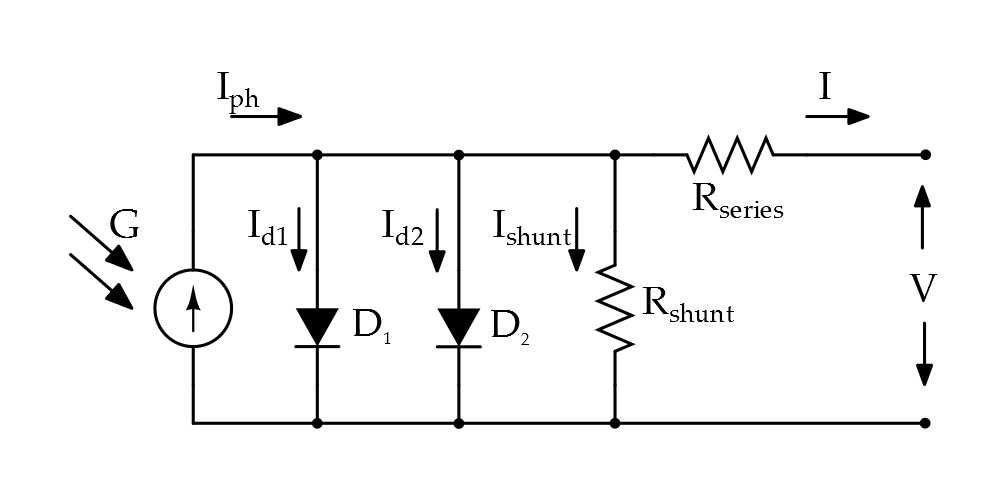
\includegraphics[width=\textwidth]{images/Double_diode_model}
  \caption{ Double diode model for a solar cell (adapted from \cite{pv_education_org}) }
  \label{fig:Double_EQu_cell}
  \end{center}
  \end{figure}
  
The equation of the double diode model under illumination is given by:  

  \begin{equation}
   \begin{aligned}
    I = I\textsubscript{ph} - I\textsubscript{dark} - I\textsubscript{shunt} = I\textsubscript{ph} -  I\textsubscript{s1} (e^{\frac{eV}{\textit{k}T}}-1) - I\textsubscript{s2} (e^{\frac{eV}{2\textit{k}T}}-1)- \dfrac{V+IR\textsubscript{series}}{R\textsubscript{shunt}}
     \label{eq:equ_current_double}
    \end{aligned}
    \end{equation}
  
\subsection{Equivalent DSCs model}\label{sec:eDDM}

It has normally been found that \ac{DSCs} do not conform to the typical I-V curves obtained from transmission line model and ladder circuit\cite{yong2008modeling}. \ac{DSCs} are often modelled with circuits similar to conventional \textit{pn}-junction solar cell ( Section~\ref{sec:SDM} and ~\ref{sec:DDM}), however even these representations fail to correspond to experimentally obtained values.

A standard \ac{DSCs} typically contains three interfaces formed by FTO/TiO\textsubscript{2}, TiO\textsubscript{2}/dye/ electrolyte, and electrolyte/Pt-FTO as depicted in the Figure ~\ref{fig:Cell_Cycle} on page ~\pageref{fig:Cell_Cycle}. The equivalent circuit below (Figure ~\ref{fig:dsc_eq_ckt}) accounts for these interfaces. The interfacial charge transfer at the $TiO_{2}$/ dye/ electrolyte is represented by a rectifying diode(D\textsubscript{1}) and a double-layer capacitance (C\textsubscript{i}). A recombination diode D\textsubscript{2} is employed to denote the interfacial charge recombination losses to both the dye cation and the redox electrolyte. Parallel resistive losses across the cell including leakage current is indicated by R\textsubscript{Shunt}. The photo-generated current I\textsubscript{ph} is in parallel with the diodes and C\textsubscript{i}. An inductive recombination pathway as a result of a charge-transfer current is incorporated into the circuit, consisting of a recombination resistance ( R\textsubscript{rec} in series with the an inductor (L). The charge-transfer resistance and interfacial capacitance at the FTO electrode and electrolyte/Pt-FTO interface are represented by R\textsubscript{E} and C\textsubscript{E}, and R\textsubscript{CE} and C\textsubscript{CE} respectively. The Nernst diffusion of the carrier transport by ions within the electrolyte is denoted by the Warburg impedance (W). A resistance element {R\textsubscript{Series}, designates the bulk and contact resistive losses present in a practical \ac{DSCs}, such as the sheet resistance of the FTO glass, contact resistance etc. The I-V characteristics based on the equivalent circuit model in figure ~\ref{fig:dsc_eq_ckt} is described in equations ~\ref{eq:equ_current_dSC} \cite{yong2008modeling}.
    


 \begin{figure}[H]
  \begin{center}
	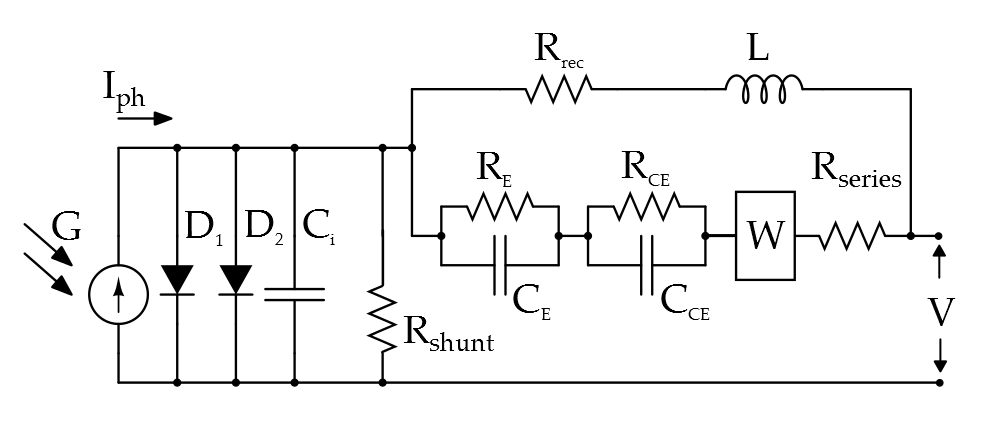
\includegraphics[width=1.0\linewidth]{images/dsc_eq_ckt}
	\caption{Equivalent circuit for DSCs (adapted from \cite{yong2008modeling})  }
	\label{fig:dsc_eq_ckt}
  \end{center}
  \end{figure}

 \begin{equation}
  \begin{aligned}
    I = I\textsubscript{ph} -  I\textsubscript{s1} (e^{\frac{eV}{\textit{mk}T}}-1) - I\textsubscript{s2} (e^{\frac{eV}{2\textit{mk}T}}-1)- (V+IZ)(\textit{j}{\omega}C\textsubscript{i}+\frac{1}{R\textsubscript{Shunt}}) 
     \label{eq:equ_current_dSC}
  \end{aligned}
 \end{equation}
    
 \begin{equation}
  \begin{aligned}
     I\textsubscript{ph} =\int{qF(\lambda)[1-r(\lambda)]IPCE(\lambda)d\lambda} = \int{qF(\lambda)\Phi(\lambda)d\lambda}  
  \end{aligned}
 \end{equation}
 
  \begin{equation}
   \begin{aligned}
     Z={\dfrac{1}{{\frac{1}{(R\textsubscript{rec}+\textit{j}{\omega}L)}}+{\frac{1}{Z\textsubscript{S}}}}} 
   \end{aligned}
  \end{equation}
  
 \begin{equation}
   \begin{aligned}
    Z\textsubscript{S}={\dfrac{1}{{\textit{j}{\omega}C\textsubscript{E}}+{\frac{1}{R\textsubscript{E}}}}}+{\dfrac{1}{{\textit{j}{\omega}C\textsubscript{CE}}+{\frac{1}{R\textsubscript{CE}}}}}+W+R\textsubscript{S}
   \end{aligned}
  \end{equation}
  
   \begin{equation}
     \begin{aligned}
     W = \sigma{\omega^{-1/2}}(1-\textit{j})
     \end{aligned}
    \end{equation}
    
Where T is the absolute temperature, $\omega$ is the angular frequency, $\sigma$ is the Warburg coefficient, $F(\lambda)$ and  $IPCE(\lambda)$ are the incident photon flux density and the incident photon-to-current conversion efficiency at wavelength $\lambda$ respectively, $r(\lambda)$ is the incident light losses due to the light absorption and reflection by the FTO glass, and $\Phi(\lambda)$ is the quantum yield \cite{yong2008modeling}.\newline

  




% %**Pictures and text about losses in the light absorption in the cell **

% %**talk ABOUT STABILITY OF dcs with change in temperature **

\section{Maximum Power Point Tracking(MPPT)}


Despite all the advantages presented by the generation of energy through the use of solar cells the efficiency of energy conversion is currently low (the best commercial solar module is only 21.5\% efficient) and the initial cost for its implementation is still considered high. Thus it becomes pertinent to use various techniques to extract the maximum power from these cells, in order to achieve maximum efficiency in operation. It should be noted that there is only one maximum power point (MPP) for a given panel, and this varies according to climatic and irradiation conditions\cite{eltawil2013mppt}.

To overcome this problem, several methods for extracting the maximum power have been proposed and many comparative studies have been published in literature  \cite{chu2009robust}, \cite{clark2006power}, \cite{eltawil2013mppt}, \cite{esram2007comparison}, \cite{faranda2008energy}, \cite{houssamo2013experimental}, \cite{ngan2011study} and \cite{reza2013classification}. 

\subsection{Perturb and Observe (PnO) Method } \label{sec:pno_sec}


    \begin{figure}[H]
       \begin{center}
       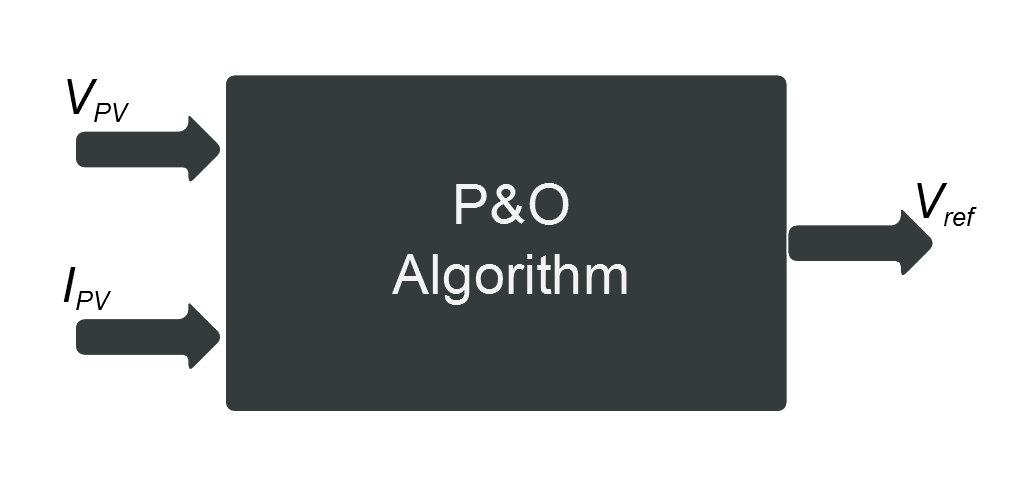
\includegraphics[width=0.4\textwidth]{images/PnO_block}
       \caption{ Black box model for the Perturb and Observe Algorithm }
       \label{fig:PnO_block}
       \end{center}
       \end{figure}
       
  The \ac{PnO} Method is most widely used in \ac{MPPT} because of  its simple structure and it requires only few parameters. Figure ~\ref{fig:PnO_flow}  shows the flow chart of \ac{PnO} method. It perturbs the PV array's terminal voltage periodically and then it compares the PV output power with that of the previous cycle of perturbation. When PV power and PV voltage increase at the same time and vice versa, a perturbation step size, ${\Delta}$D will be added to the duty cycle, D to generate the next cycle of   perturbation in order to force the operating point moving towards the \ac{MPP}. When PV power increases and PV voltage decreases and vice versa, the perturbation step will be subtracted for the next cycle of perturbation. This process will be carried on continuously until \ac{MPP} is reached. However, the system will oscillate around the \ac{MPP} throughout this process, and this will result in loss of energy. These oscillations can be minimised by reducing the perturbation step size but it significantly slows down the \ac{MPP} tracking system also leading to loss of energy \cite{ngan2011study}. \ac{PnO} is also not suitable when the light intensity changes rapidly. \\ %** explain why not suitable**
  
  \begin{figure}[H]
    \begin{center}
    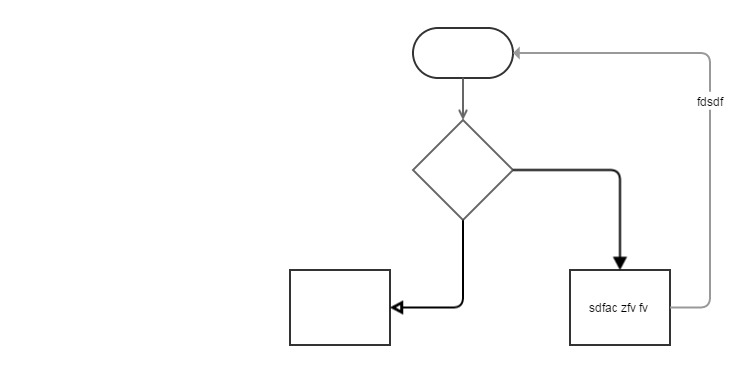
\includegraphics[width=\textwidth]{images/pno_flow}
    \caption{Flow chart for the Perturb and Observe Method }
    \label{fig:PnO_flow}
    \end{center}
    \end{figure}
  
  \subsection{Incremental Conductance Method (ICM) } \label{sec:icm_sec}
  
  \begin{figure}[H]
         \begin{center}
         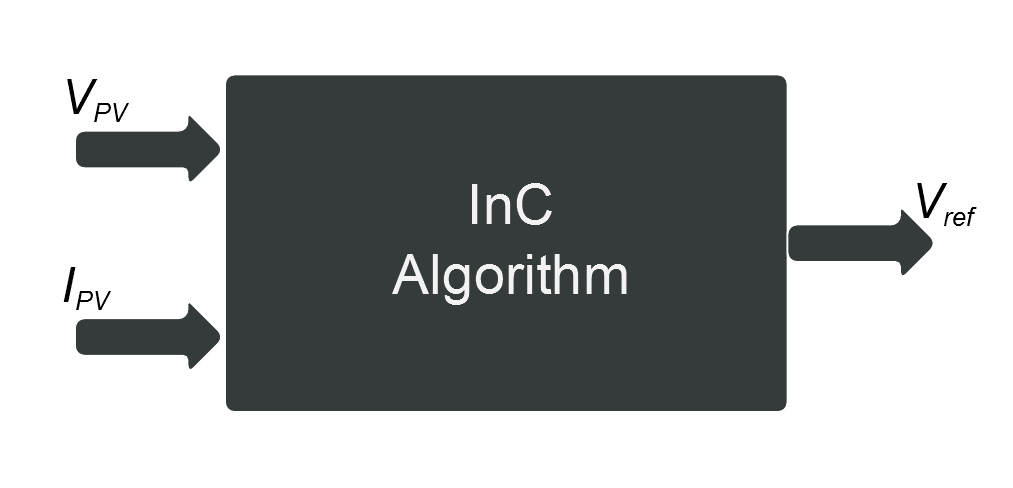
\includegraphics[width=0.4\textwidth]{images/inC_block}
         \caption{ Black box model for the Incremental Conductance Algorithm }
         \label{fig:inC_block}
    \end{center}
  \end{figure}
  
  The  solar array terminal  voltage  can  be  adjusted relative to the MPP voltage by measuring the incremental and instantaneous  array  conductance (dI/dV and I/V, respectively). The algorithm is based on the fact that at the \ac{MPP}, the derivative of the cell's power is zero. Although  the  incremental  conductance method offers good performance under rapidly changing atmospheric  conditions, four  sensors  are  required to perform the computations. The  drawback is that sensor devices require  more  conversion  time  thus  resulting in a large amount of power loss \cite{gomathy2012design}. In addition to the above drawback, the \ac{ICM} suffers the same limitations as \ac{PnO} method namely, for rapid tracking larger step sized must be utilised which results in the oscillation around the \ac{MPP}. \\
  
   \begin{figure}[H]
      \begin{center}
      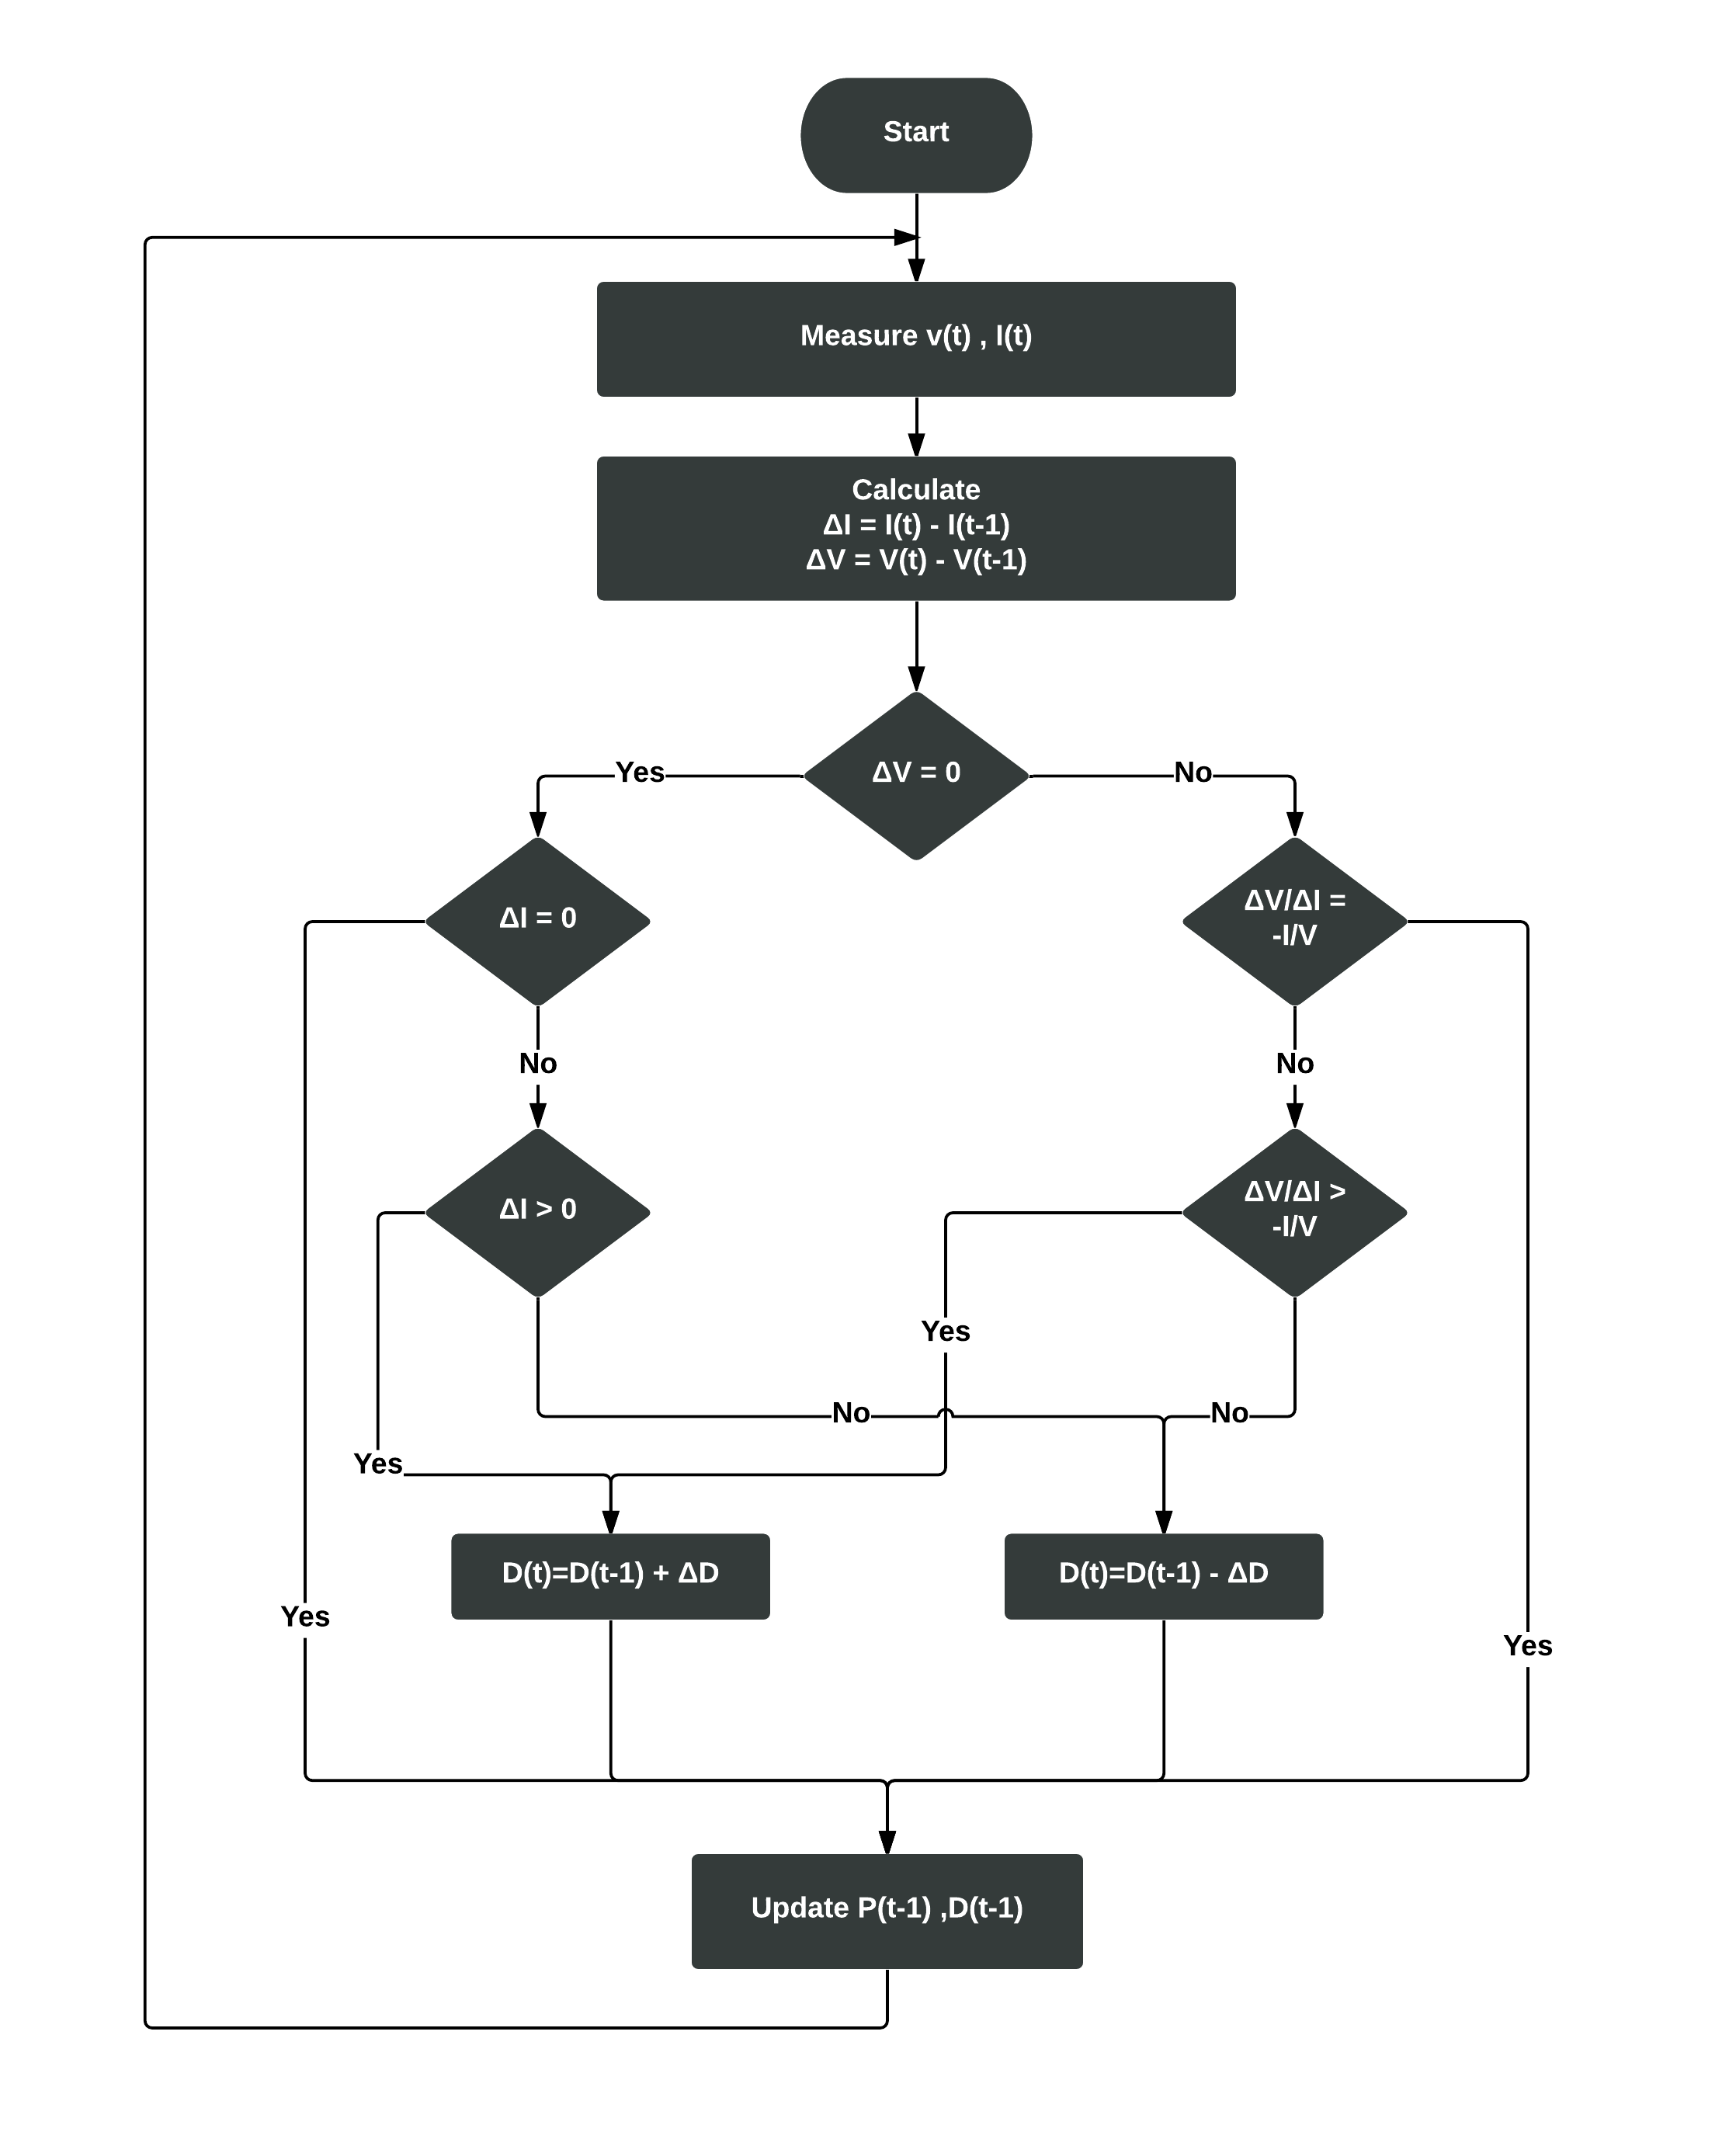
\includegraphics[width=\textwidth]{images/INc_flow}
      \caption{ Flow chart for the Incremental Conductance Method}
      \label{fig:inCflow}
      \end{center}
      \end{figure}
      
  \subsection{Fractional Open Circuit Voltage (FOCV) Method  } \label{sec:focv_sec}
  
   \begin{figure}[H]
           \begin{center}
           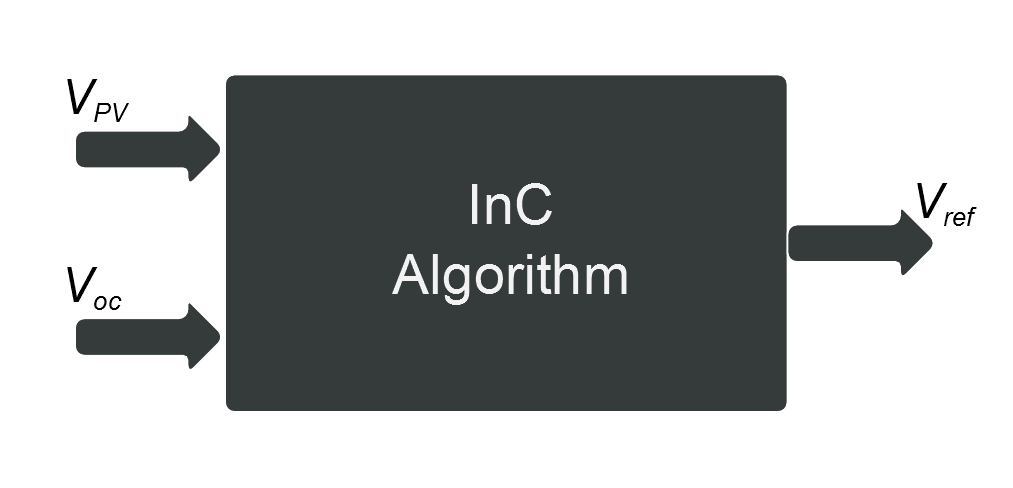
\includegraphics[width=0.4\textwidth]{images/Frac_block}
           \caption{ Black box model for the Incremental Conductance Algorithm }
           \label{fig:Frac_block}
      \end{center}
    \end{figure}
  This is a method based on the linear relationship between output voltage of the PV array at the \ac{MPP}, V\textsubscript{MPP} and the PV array's open circuit voltage, V\textsubscript{OC} in under varying temperature and solar irradiance. \\
  
  \begin{equation}
    \begin{aligned}
  V\textsubscript{MPP}\approx k\textsubscript{i}V\textsubscript{OC}
  \label{eq:equ_fracoc}
  \end{aligned}
  \end{equation}
  
  Constant value of k\textsubscript{i} is dependent on the characteristics of PV array. Generally, it has to be computed empirically in order to determine the V\textsubscript{MPP} and V\textsubscript{OC} for varied temperatures and solar irradiances. The value of k\textsubscript{i} ranges from 0.73 to 0.80  for most PV modules over a temperature range of 0 to 60$^\circ$C.Figure ~\ref{fig:focflow} describes the operation of a \ac{FOCV}, the PV array is temporarily isolated from \ac{MPPT},then the open circuit voltage, V\textsubscript{OC} is measured periodically by shutting down the power converter momentarily. The \ac{MPPT} calculates V\textsubscript{MPP} from the pre-set value of k\textsubscript{i} and the calculated value of V\textsubscript{OC}. Then, the array's voltage is varied until V\textsubscript{MPP} is  reached . The shut-down of power converter periodically will incur temporary loss of power which in turn leads to a situation where power extracted will not be the maxima. Since it is an approximation, the PV array will never reach the \ac{MPP}. Even though this technique is very easy and cheap for implementation; due to the fact true \ac{MPP} is never reached, there is always a loss in power during operation\cite{ngan2011study}.
  
  \begin{figure}[H]
        \begin{center}
        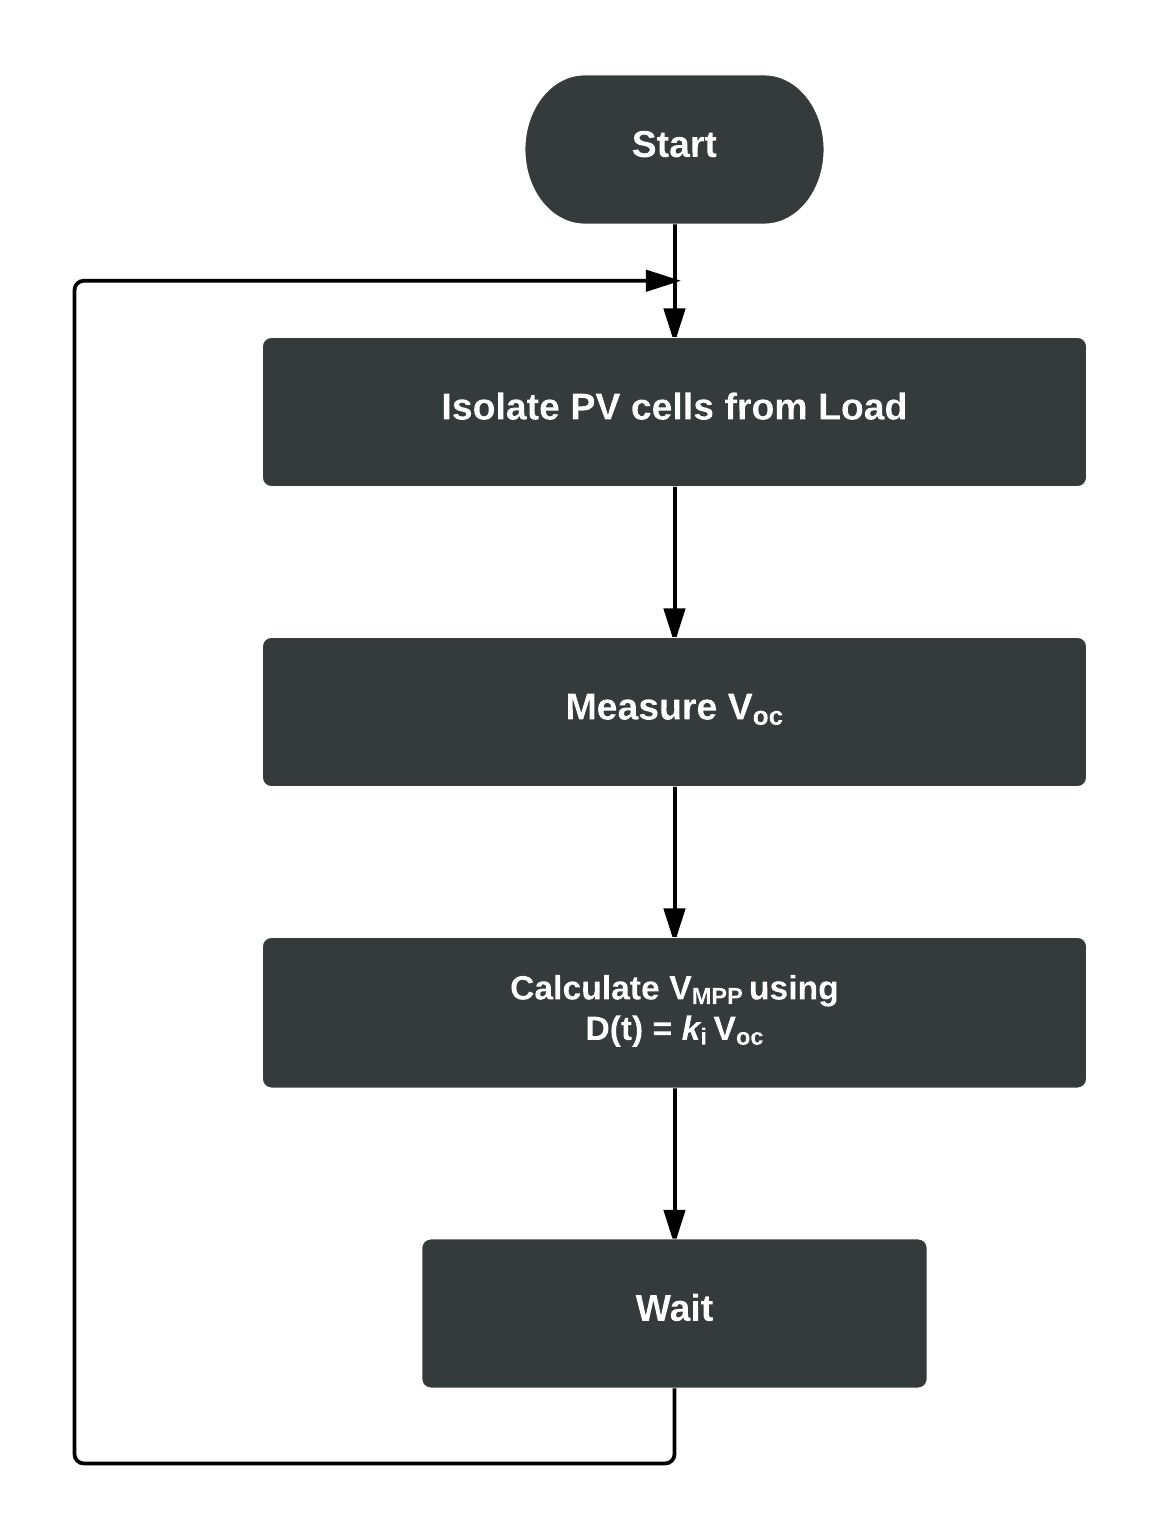
\includegraphics[width=0.5\textwidth]{images/Vopen_circuit_Flow}       %Frac_Flow}
        \caption{ Flow chart for the Fractional Open Circuit Voltage Method (adapted from \cite{reza2013classification})}
        \label{fig:focflow}
        \end{center}
        \end{figure}
  
\subsection{Other algorithms}
  \begin{itemize}
  \item {\bf Fixed duty cycle}: The fixed duty cycle represents the simplest of the methods and it does not require any feedback, where the load impedance is adjusted only once for the maximum power point and it is not adjusted again.
  \item {\bf Pilot cell}: In the pilot cell MPPT algorithm, the constant voltage or current method is used, but the open-circuit voltage or short-circuit current measurements are made on a small solar cell, called a pilot cell, that has the same characteristics as the cells in the larger solar array. The pilot cell measurements can be used by the MPPT to operate the main solar array at its MPP, eliminating the loss of PV power during the V\textsubscript{OC} or I\textsubscript{sc} measurement
  \item {\bf Fractional short-circuit current }: Under varying atmospheric conditions, I\textsubscript{MPP} is approximately linearly related to the I\textsubscript{SC} of the PV array. \newline
    \begin{equation}
      \begin{aligned}
    I\textsubscript{MPP} \approx k\textsubscript{j}I\textsubscript{SC}
    \label{eq:equ_fracoc_cur}
    \end{aligned}
    \end{equation}
   \item {\bf Fuzzy logic controller} (FLC):They have the advantages of working with imprecise inputs, it does not need an accurate mathematical model and it can handle non-linearity as well \cite{messai2011maximum}.However their effectiveness depends a lot on the presence of an expert knowledge; conversely, in the absence of such knowledge, their design is usually slow and not optimised. 
  \end{itemize} 
  







\section{Machine Learning }
This section discusses about Search optimization in order to lock on the  V\textsubscript{MP} and I\textsubscript{MP} as efficiently as possible.\\

Much like Embedded systems, Machine Learning encompasses various disciplines, predominantly Computer science but also statistics, Mathematics, Finance etc. \cite{marsland2011machine}; with applications ranging from predicting emergency-room wait-times \cite{connelly2004discrete} to High Frequency Stock-trading. Simply put, Machine learning is about algorithms that build models which adapt or modify their response in order to get closer to the correct output. These models are automatically created and they constantly evolve based on input vectors, as opposed to having a hard coded decision tree.\\

If the input vectors provided to the algorithm in its training set are 'labelled' , then this kind of learning is called \textbf{Supervised learning}. Where correct or expected responses are provided based on this the algorithm is able to generalise the out put for all possible outputs. In the other end of the spectrum is \textbf{Unsupervised learning} in which the algorithm is left to find hidden structures in a set of data that doesn't have any labels or that all have the same label. In our application we know the input is V\textsubscript{OC} and what the expected Output (V\textsubscript{MPP})is supposed to be. This constitutes as  labelling and hence classified as Supervised learning.
 
\subsection{Regression Modelling }

We use regression analysis when we want to predict one variable from another. The most basic form of regression is called simple regression, where one independent variable and one dependent variable exists and where linear trend is to be predicted. In regression, we attempt to determine the magnitude of the relationship between a set of independent variables and the dependent variable. Independent variable(X), also called the predictor variable, influences the Dependent variable(Y),sometimes called the response variable  \cite{lenarreg2006}.\\

A regression model is a formal way of stating:
\begin{itemize}
\item The tendency of the response variable(Y) to vary with the predictor variable(X).
\item A scattering of points around some statistical relationship.
\end {itemize}

Equation for a line can be written as:

\begin{equation}
\begin{aligned}
  y= mx + b 
\label{eq:Line_equ}
\end{aligned}
\end{equation}

The linear regression model(for observation i = 1, . . . , N) can we written as:

\begin{equation}
\begin{aligned}
  Y\textsubscript{i}= \beta\textsubscript{0}+\beta\textsubscript{1}X\textsubscript{i} +\epsilon\textsubscript{i}
\label{eq:Line_equ_exp}
\end{aligned}
\end{equation}

\begin{itemize}
\item $\beta\textsubscript{0}$ is the mean of the population when X is zero -the Y intercept.
\item $\beta\textsubscript{1}$ is the slope of the line, the amount of increase in Y brought about by a unit increase $(X^{'}= X + 1)$ in X.
\item \textbf{$\epsilon\textsubscript{i}$} is the random error, specific to each observation.
\item the goal is to find $\beta\textsubscript{0}$ and $\beta\textsubscript{1}$ such that $\sum\limits_{i=1}^n \epsilon\textsubscript{i}^2$ is minimised.
\end {itemize}
A large number of methods and procedures have been developed to estimate the parameters of a model, the simplest being :\\

\begin{equation}
	\begin{aligned}
		\beta\textsubscript{1}= \dfrac{\sum (X\textsubscript{i} - \bar{X})(Y\textsubscript{i} - \bar{Y})}{\sum (X\textsubscript{i} - \bar{X})^2} 
	\label{eq:B1_calculus}
	\end{aligned}
\end{equation}

\begin{equation}
	\begin{aligned}
		\beta\textsubscript{0}= \bar{Y}-\beta\textsubscript{1}\bar{X} 
	\label{eq:B0_calculus}
	\end{aligned}
\end{equation}

\begin{figure}[H]
  \begin{center}
  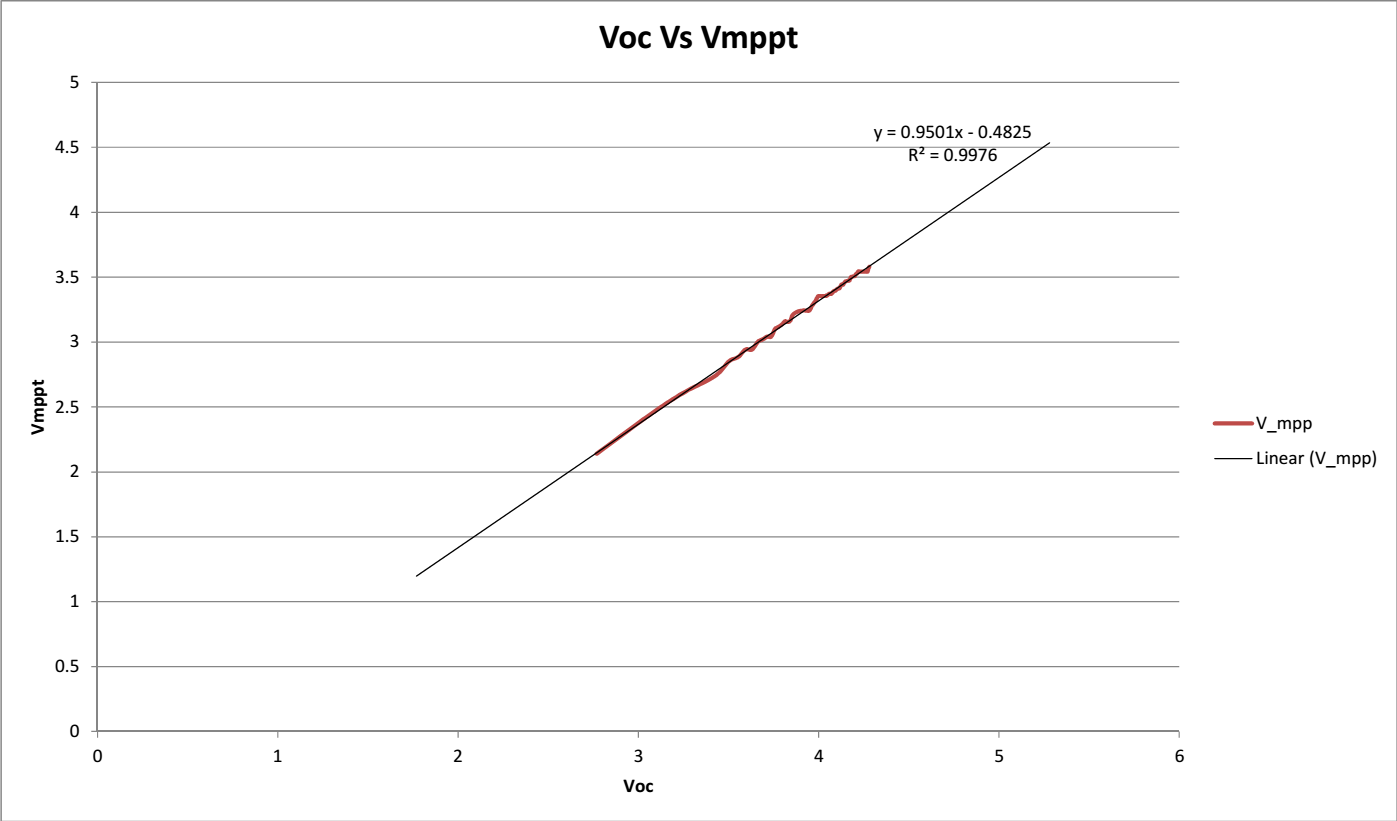
\includegraphics[width=\textwidth]{images/Reg_line}
  \caption{ Example for Linear regression }
  \label{fig:linear_regression}
  \end{center}
  \end{figure}


In Figure ~\ref{fig:linear_regression} the points in red represent $V_{MPP}$ for a given $V_{OC}$. It is clear from the graph that the relationship between $V_{MPP}$ and $V_{OC}$ is linear, this is also supported in various literature (\cite{reza2013classification},\cite{esram2007comparison},etc.) and forms the basis of \ac{FOCV} method. The trend line in black (obtained via Regression Modelling) tells us about the slope of the line ($\beta\textsubscript{1}$) and the Y intercept. It also provides the $R^{2}$ value of the fit equal to 0.9976, indicating the goodness of fit. $R^{2}$ is a measure of how close the regression line is to the data points, with $R^{2} = 1 $ signifying that the model/regression-line perfectly fits the data \cite{Jim_R_squared}.


\subsection{Pattern search}


Finding the maxima or minima ( collectively known as extrema) of a first order single variable function can easily be found by equating the derivative of this function to zero. However finding the derivative of certain functions is not always easy or possible. In such conditions, various search techniques are used to find the maxima or minima  in a uni-modal ( a uni-modal function contains only one minimum or maximum on the specified interval) continuous function over an interval without using derivatives \cite{seiler1989numerical}. \ac{GSSA} is one such search method. The algorithm derives its name from the Golden ratio (0.61803...)\\

Two numbers are said to be in the Golden ratio if their ratio is same as the ratio of their sum to the larger of the two quantities. Assuming $\beta > \alpha$ then this can be expressed as\cite{Gill81MurrayWright}:\\

\begin{equation}
	\begin{aligned}
		\dfrac{\alpha+\beta}{\beta}=\dfrac{\beta}{\alpha}=\phi
		\label{eq:golden_ratio1}
	\end{aligned}
\end{equation}

where ${\phi}$ is the Golden ratio whose value is given by:\\

\begin{equation}
	\begin{aligned}
		 \phi=\dfrac{\sqrt{5}-1}{2}= 0.61803398874989......
		\label{eq:golden_ratio}
	\end{aligned}
\end{equation}
 
 Assuming \textit{f(x)} to be an uni-modal function in the intervals between  \textit{a} and \textit{b}. It is very important for the extrema exists within the range to prevent misleading results. The maxima is represented by $\textit{f}(P_{\textit{max}})$ such that $a\leq P_{\textit{max}} \leq b $.
 \begin{itemize}
 
 \item Points $P_{1} \& P_{2}$ are chosen such that they satisfy:
 
\begin{equation}
	\begin{aligned}
		 P_{1}=a+(1-\phi)(b-a)
		\label{eq:golden_ratio_p1}
	\end{aligned}
\end{equation}

\begin{equation}
	\begin{aligned}
		 P_{2}=a+\phi(b-a)
		\label{eq:golden_ratio_p2}
	\end{aligned}
\end{equation}


	\item $\textit{f}(a),\textit{f}(P_{1}),\textit{f}(P_{2})$ and $\textit{f}(b)$ is computed.
	\item If $\textit{f}(P_{1}) > \textit{f}(P_{2})$ then the outer bound is discarded and replaced by $ P_{2} $ and $ P_{2}$ replaced $ P_{1}$; a new $ P_{1}$ is calculated using equation ~\ref{eq:golden_ratio_p1}.
	\item Else the lower bound is cast-off to be replaced with $ P_{1}$ and $ P_{1}$ is swapped with $ P_{2}$; with $ P_{2}$ found afresh using equation ~\ref{eq:golden_ratio_p2}.
	\item New values of either $\textit{f}(P_{1})$ or $\textit{f}(P_{2})$ are found out depending on the branch taken.
	\item  The process repeated over and over again only stopping when either the iteration count has run out or if the lower and upper bounds are close enough to be acceptably small. 
\end{itemize}

 
\begin{figure}[H]
  \begin{center}
  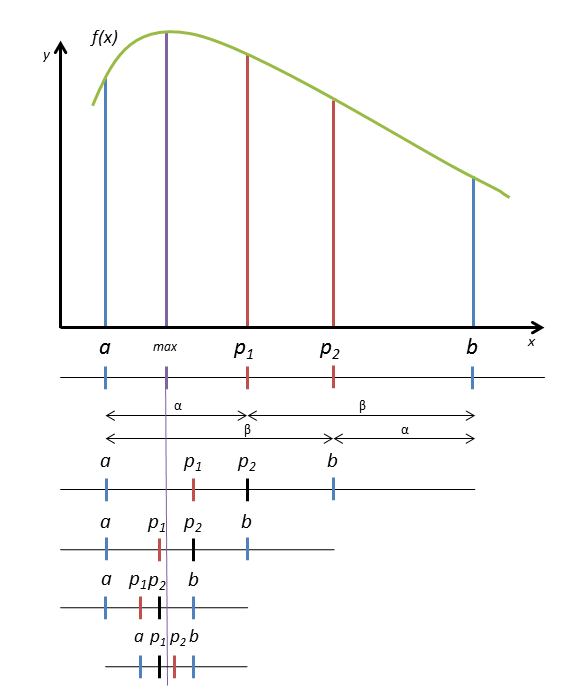
\includegraphics[width=0.92\textwidth]{images/Golden_search_curve}
  \caption{ Golden Section search algorithm }
  \label{fig:Golden_search_curve}
  \end{center}
  \end{figure}
  
The advantage of using \ac{GSSA} over other search methods is that the extrema is found in the least number of steps and every iteration requires only one additional data point. Thereby greatly reducing the complexity of the algorithm and hence the computation power and/or time required to lock-in onto the extrema.

\begin{itemize}
	 \item The blue points represent extremes of the successive
	 \item Red points  are the newly evaluated values
	 \item Black points are the already evaluated values.
 \end{itemize}


 
\begin{figure}[H]
  \begin{center}
  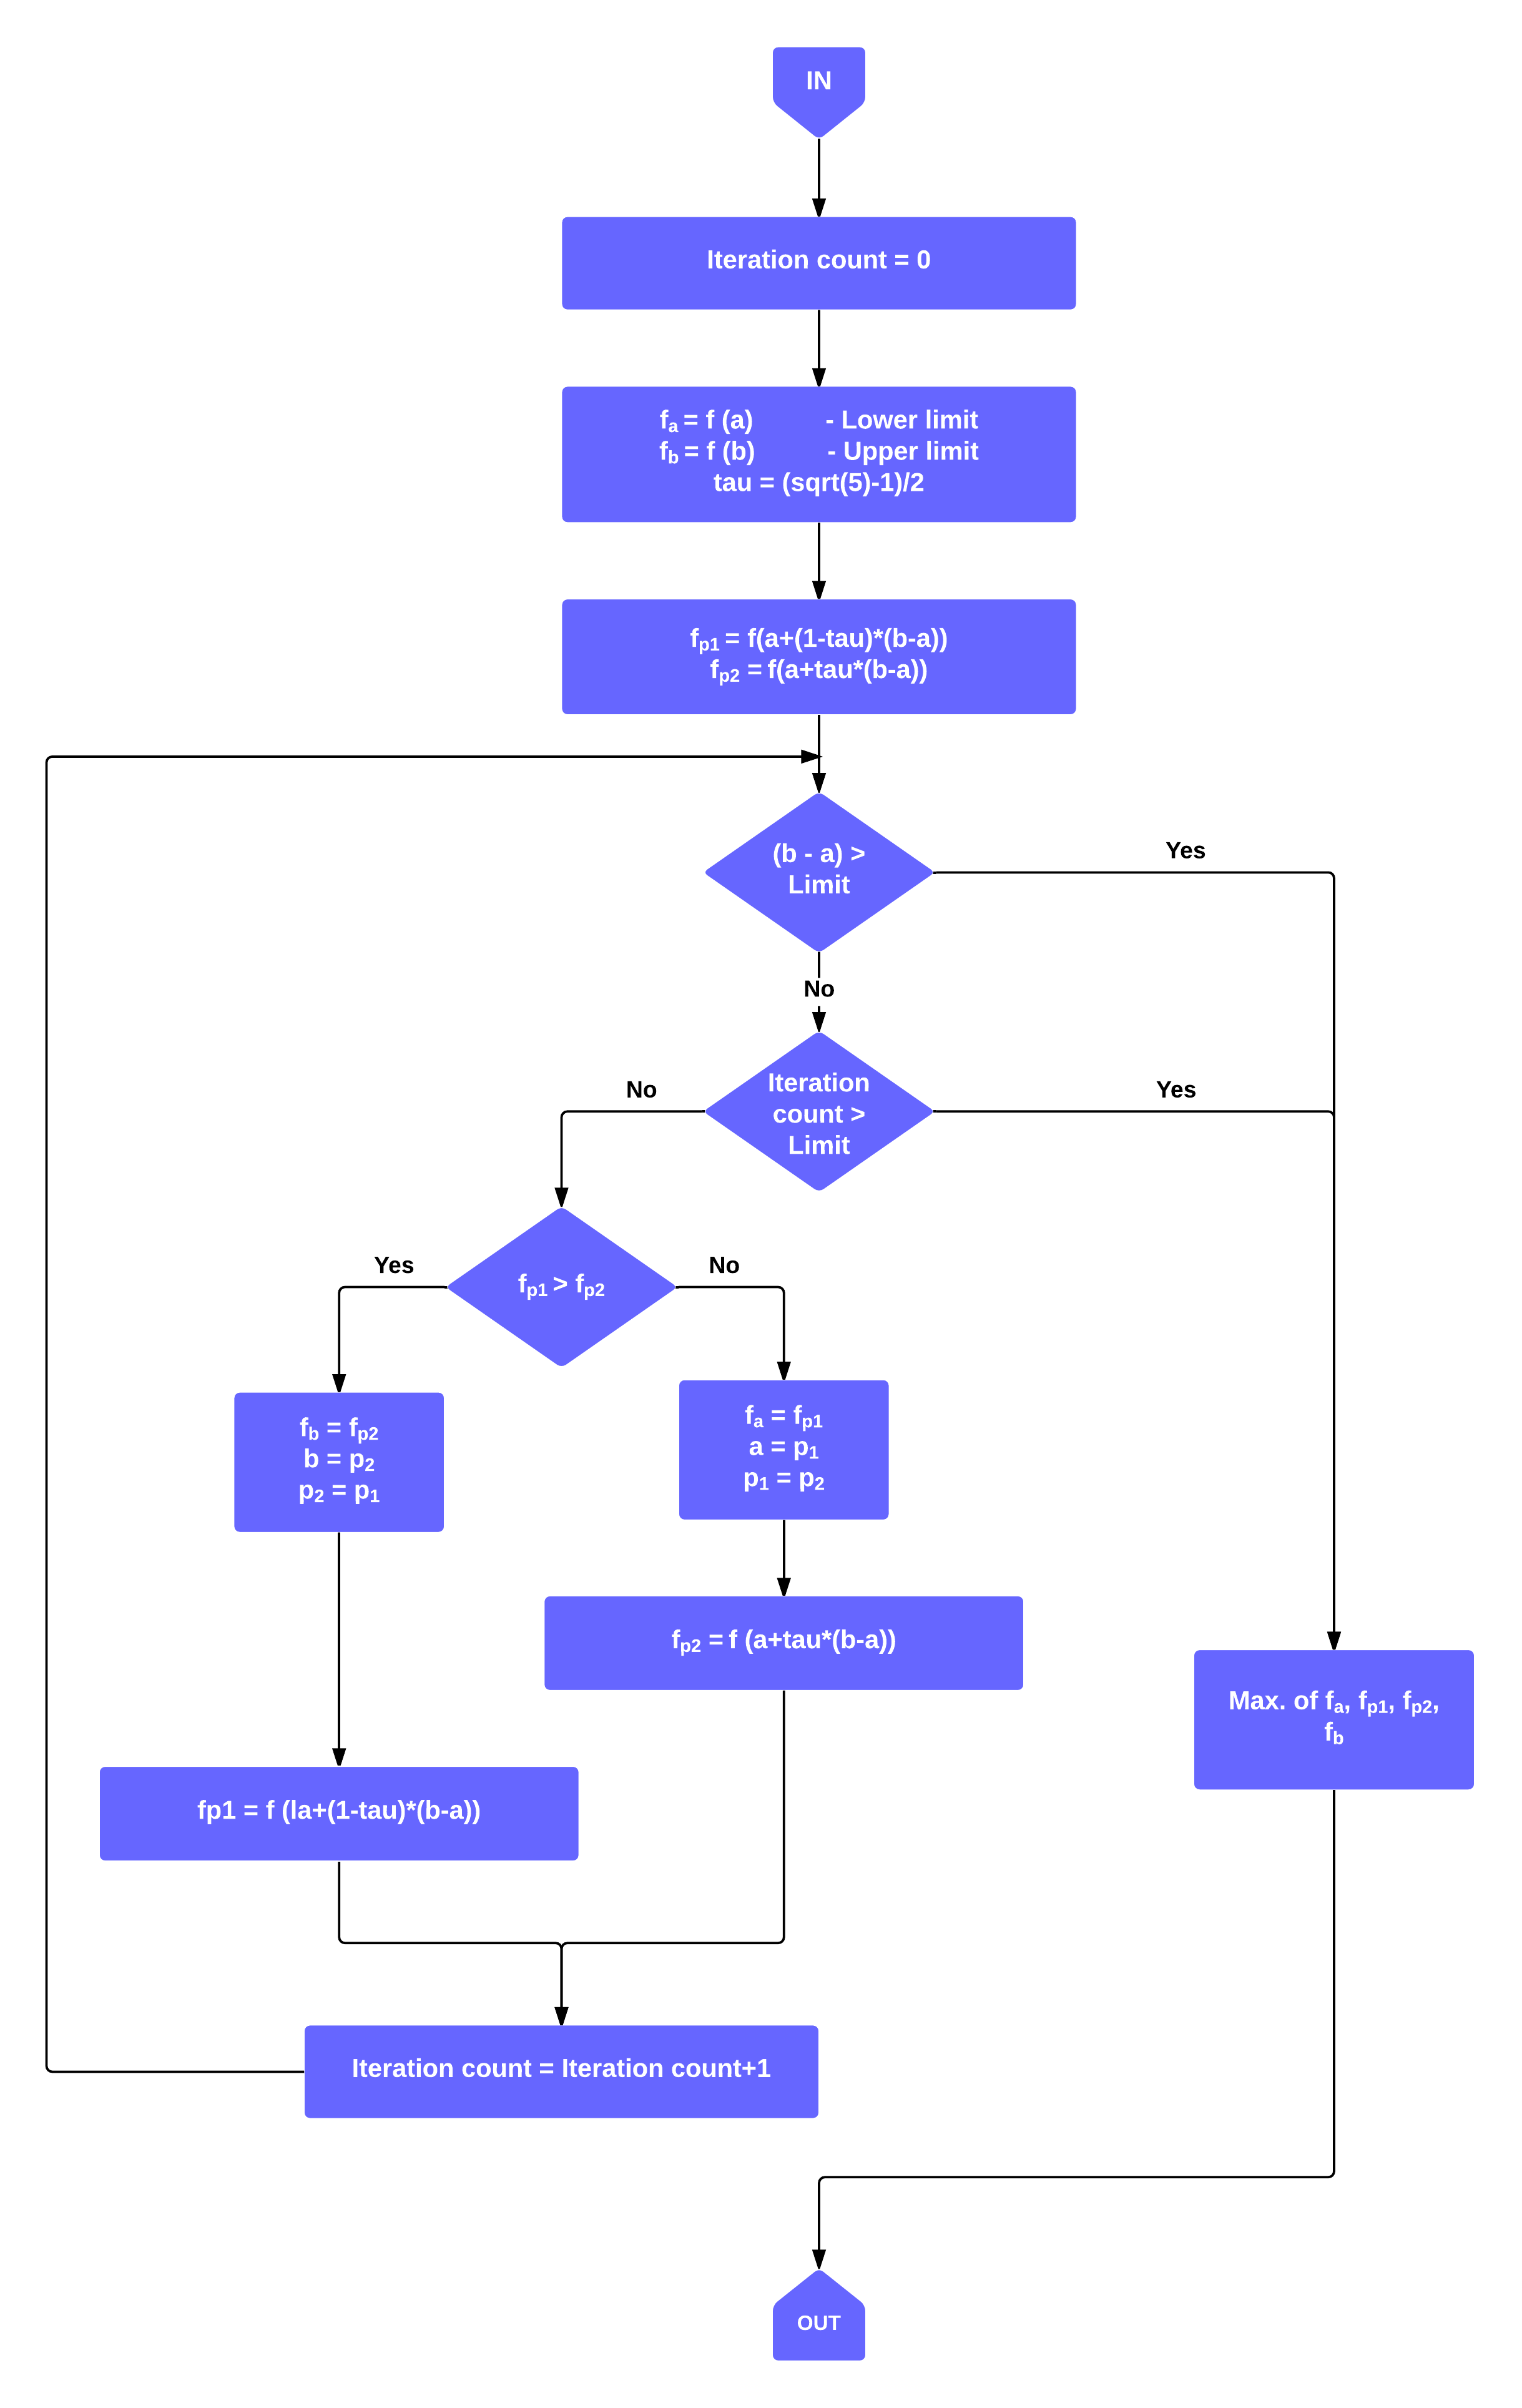
\includegraphics[width=\textwidth]{images/Golden_Search}
  \caption{ Golden Section search algorithm (modified from \cite{van1970fitting})}
  \label{fig:Golden_search}
  \end{center}
  \end{figure}
  
 
